\documentclass[print,Draft]{faosyb}
\usepackage{lipsum}
\faoset{year=2013}
\begin{document}

\addtocounter{page}{1}  % To make odd pages even and even pages odd

\frontmatter

\tableofcontents
\listofmaps
\listoftables
\listofcharts

\part*{Foreword}
\lipsum

\part*{Ack\-now\-ledgements}
\lipsum

\part*{How to use this book}
\lipsum


\mainmatter
\faoset{bgcolor=blue,icon=icons/settings}
\part[The Setting]{The\\ Setting}
\lipsum
\EndPartIntro

\section{Overview}
\label{sec:first}

\lipsum[1-4]

\begin{map}{S}{ll}
\caption{Ancient Roma  (Trajan times)}
\label{map:roma}
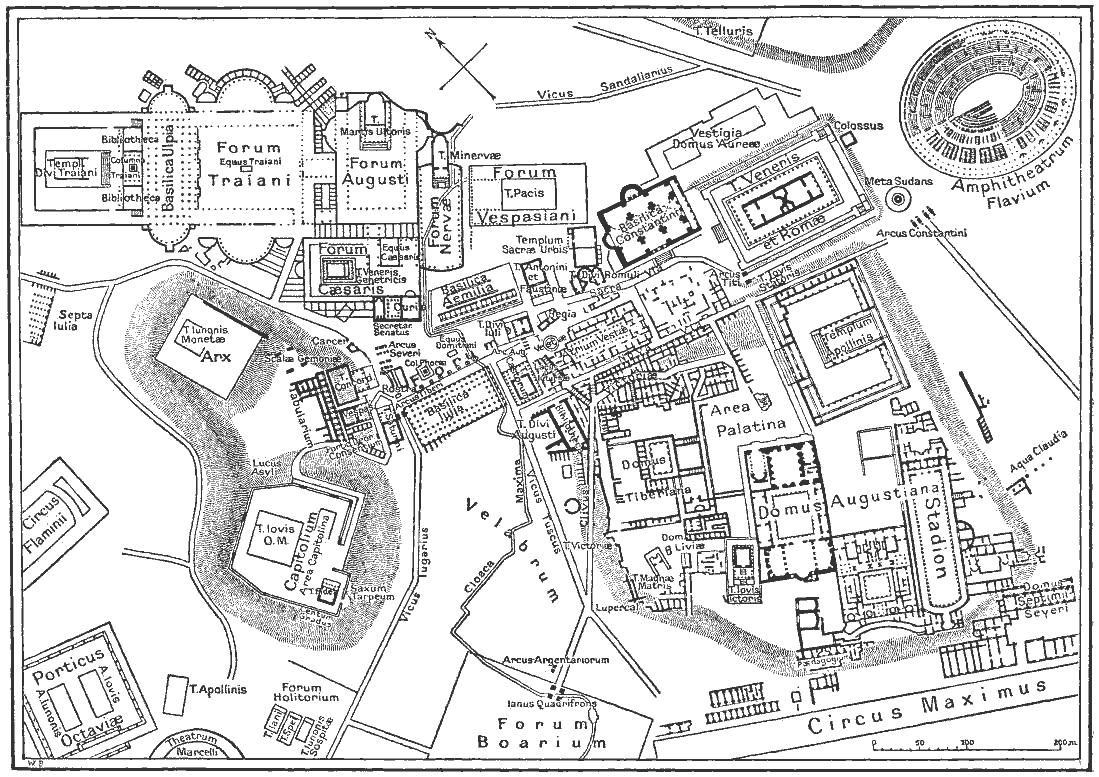
\includegraphics[width=\chartwidth,height=\chartheight]{Rome}
\source{Wikipedia}
\refMetadata{agripop}
\end{map}

\begin{map}{S}{ur}
\caption{Ancient Roma  (Trajan times)}
\label{map:roma}
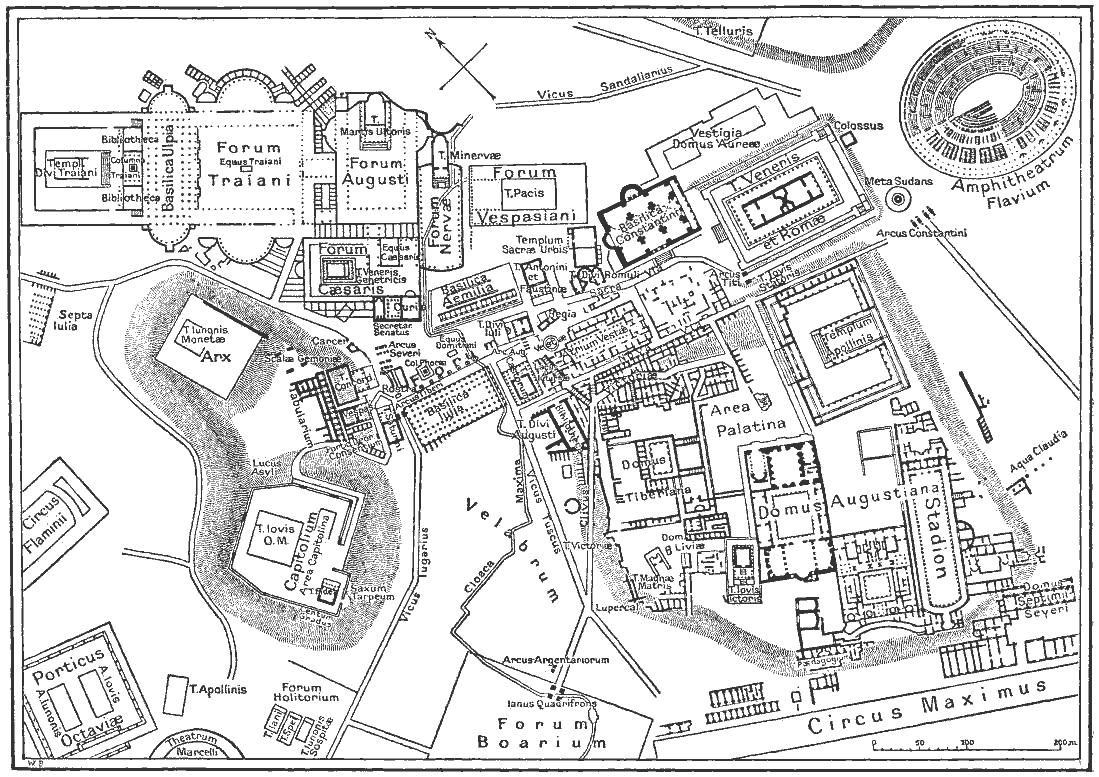
\includegraphics[width=\chartwidth,height=\chartheight]{Rome}
\source{Wikipedia}
\end{map}


\begin{map}{S}{lr}
\caption{Ancient Roma  (Trajan times)}
\label{map:roma}
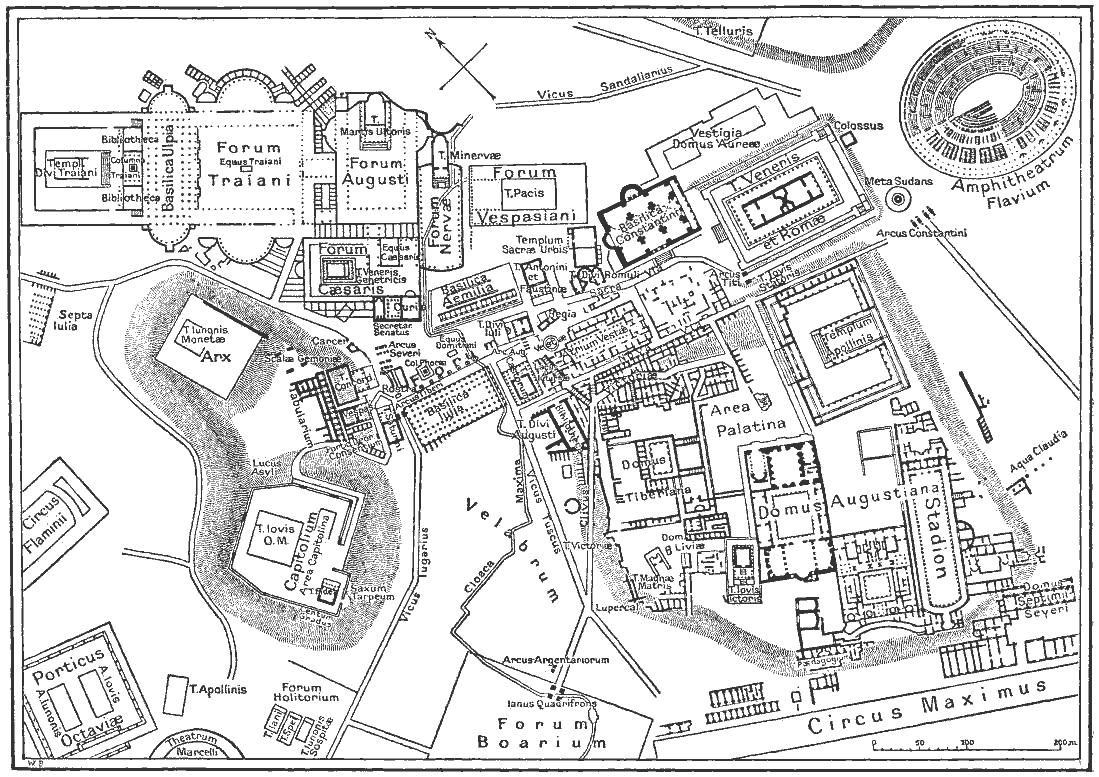
\includegraphics[width=\chartwidth,height=\chartheight]{Rome}
\source{Wikipedia}
\end{map}


\begin{map}{W}{UL}
\caption{Ancient Roma  (Trajan times)}
\label{map:roma}
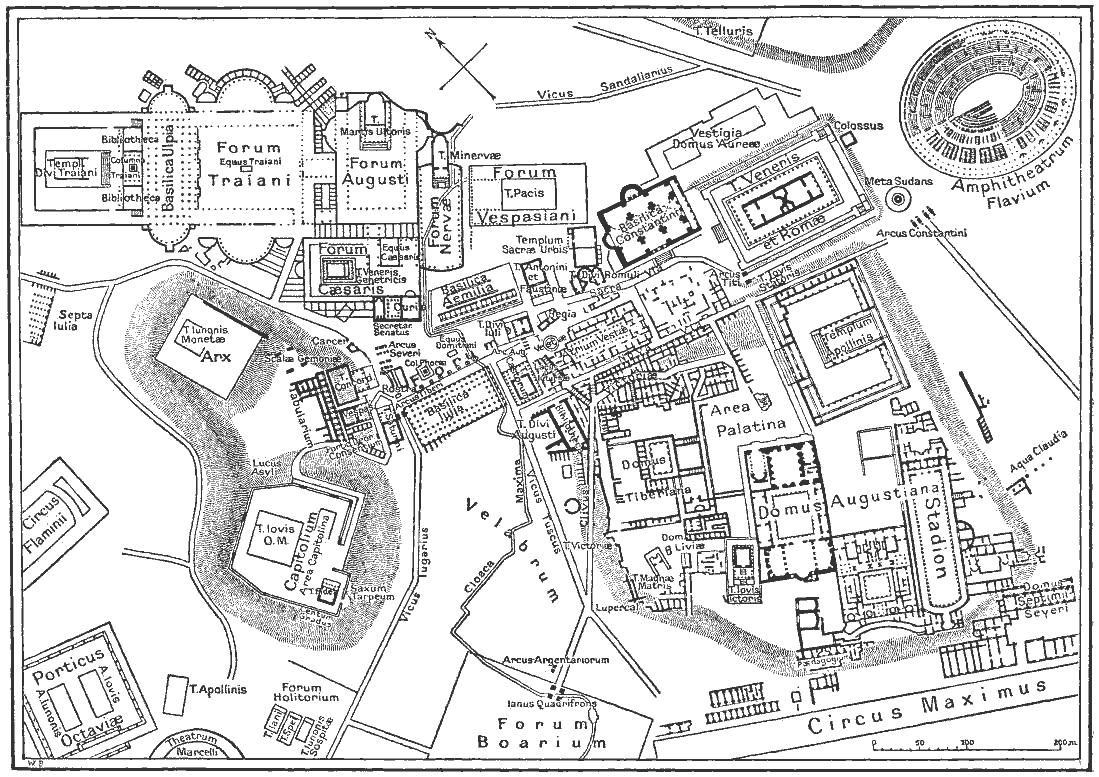
\includegraphics[width=\chartwidth,height=\chartheight]{Rome}
\source{Wikipedia}
\end{map}

\begin{chart}{S}{LL}
\caption{Incarceration ratest across countries}
\label{chart:incarceration}
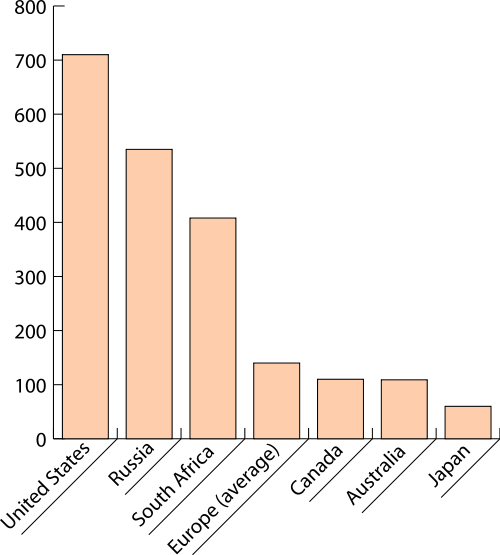
\includegraphics[width=\chartwidth,height=\chartheight]{incarceration}  
\source{Wikipedia}
\end{chart}

\begin{chart}{S}{LR}
\caption{Incarceration ratest across countries}
\label{chart:incarceration}
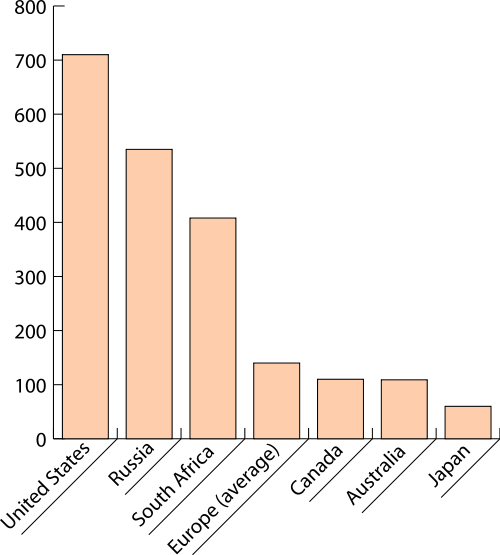
\includegraphics[width=\chartwidth,height=\chartheight]{incarceration}  
\source{Wikipedia}
\refMetadata{agripop}
\end{chart}

\section{Economy}

\begin{chart}{S}{ll}
\caption{Incarceration ratest across countries}
\label{chart:incarceration}
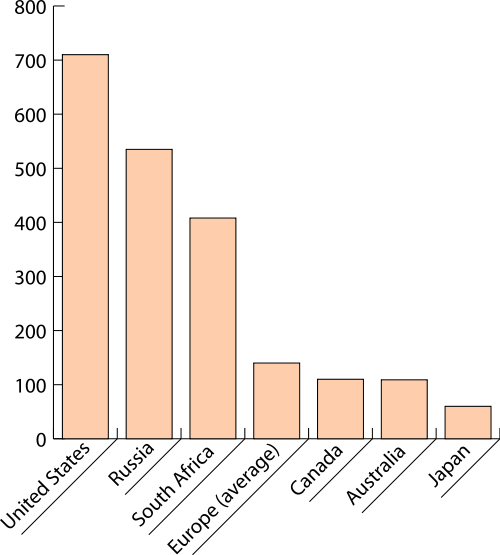
\includegraphics[width=\chartwidth,height=\chartheight]{incarceration}  
\source{Wikipedia}
\end{chart}

\begin{chart}{S}{ur}
\caption{Incarceration ratest across countries}
\label{chart:incarceration}
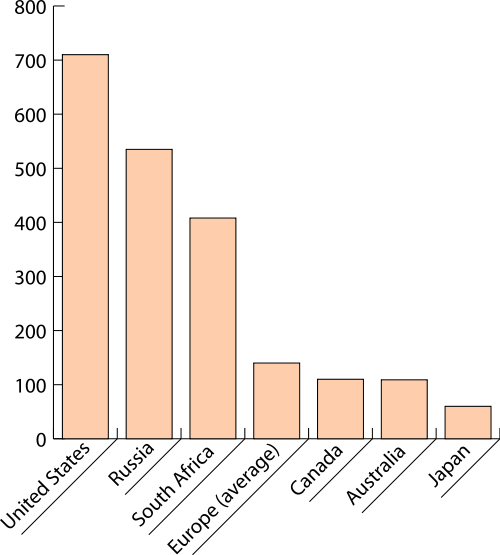
\includegraphics[width=\chartwidth,height=\chartheight]{incarceration}  
\source{Wikipedia}
\end{chart}

\begin{chart}{S}{lr}
\caption{Incarceration ratest across countries}
\label{chart:incarceration}
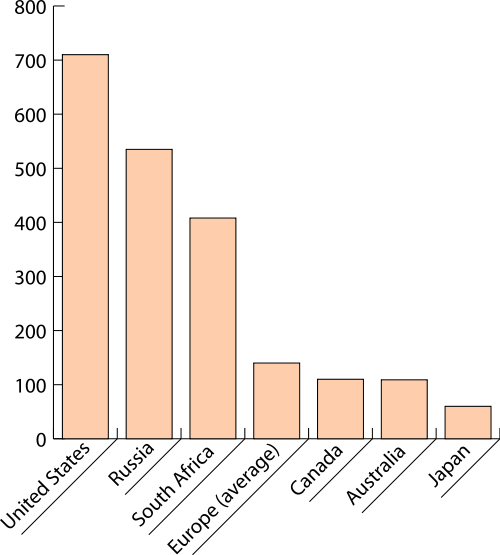
\includegraphics[width=\chartwidth,height=\chartheight]{incarceration}  
\source{Wikipedia}
\end{chart}

%\lipsum

\begin{map}{B}{UL}
\caption{Ancient Roma  (Trajan times)}
\label{map:roma}
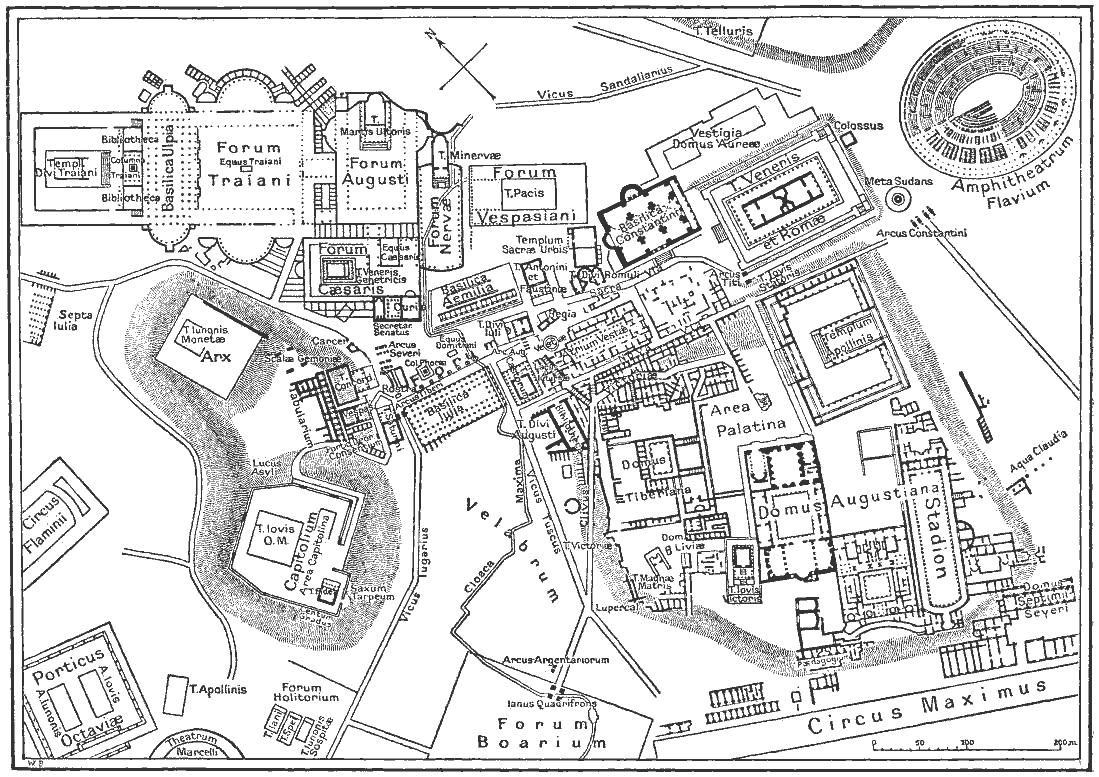
\includegraphics[width=\chartwidth,height=\chartheight]{Rome}
\source{Wikipedia}
\end{map}

\section{Land and Water}


\lipsum[1-4]

\begin{chart}{T}{ur}
\caption{Incarceration ratest across countries}
\label{chart:incarceration}
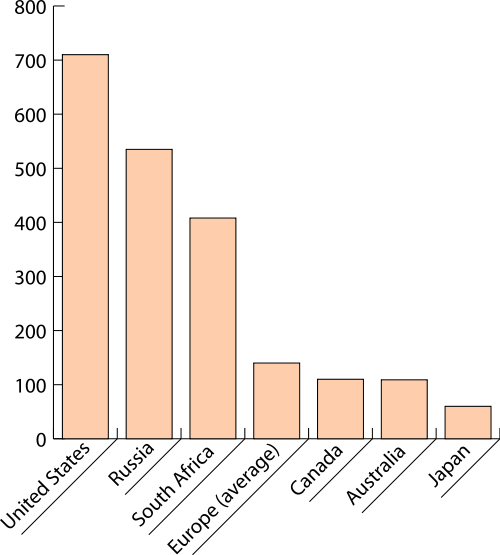
\includegraphics[width=\chartwidth,height=\chartheight]{incarceration}  
\source{Wikipedia}
\end{chart}

\begin{map}{W}{UL}
\caption{Ancient Roma  (Trajan times)}
\label{map:roma}
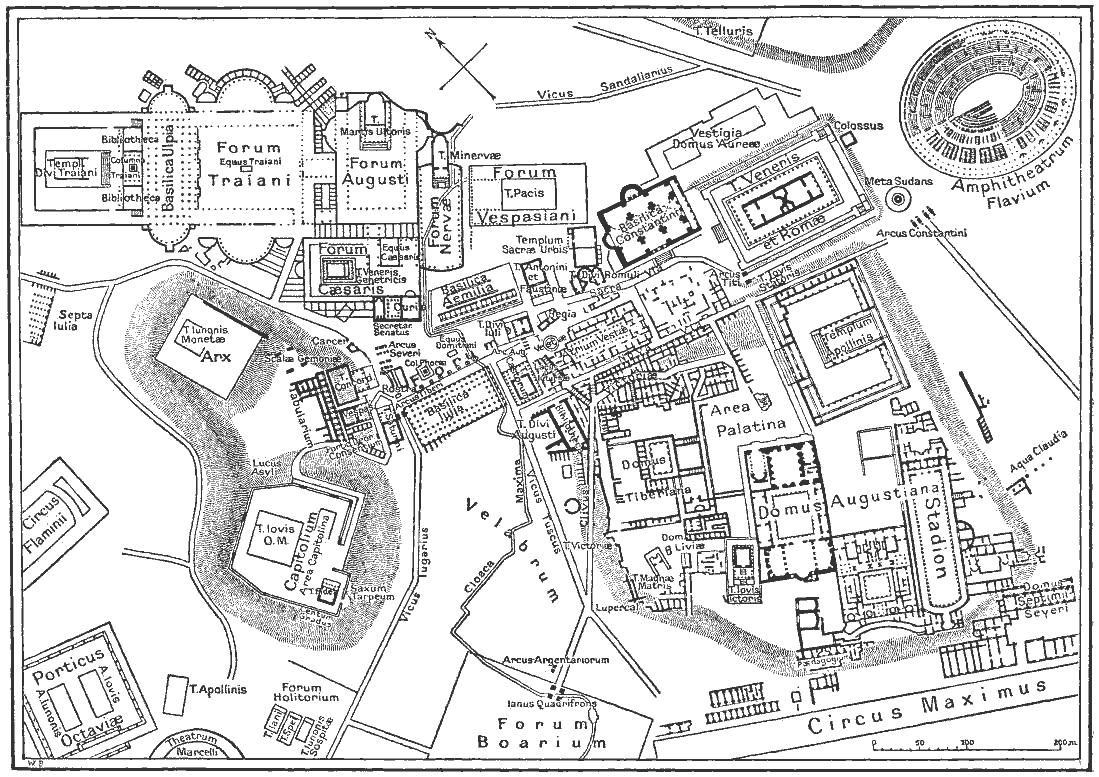
\includegraphics[width=\chartwidth,height=\chartheight]{Rome}
\source{Wikipedia}
\end{map}

\begin{map}{W}{LL}
\caption{Ancient Roma  (Trajan times)}
\label{map:roma}
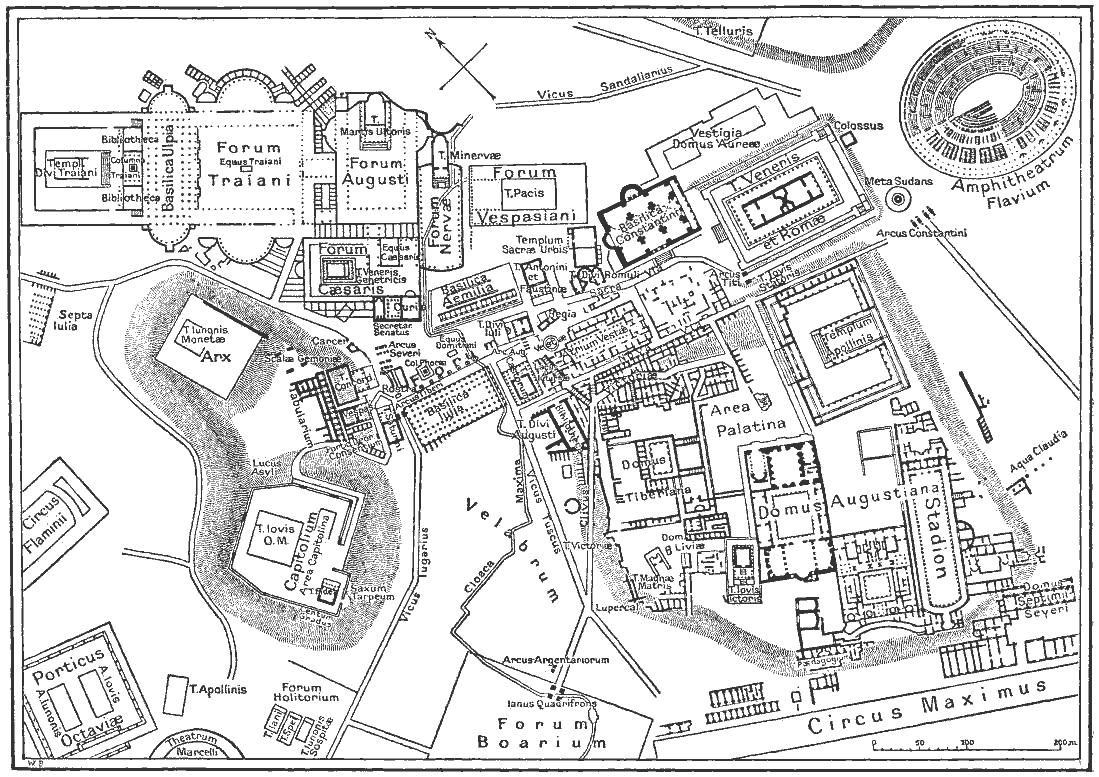
\includegraphics[width=\chartwidth,height=\chartheight]{Rome}
\source{Wikipedia}
\end{map}

\section{Labor}



\begin{chart}{S}{ur}
\caption{Incarceration ratest across countries}
\label{chart:incarceration}
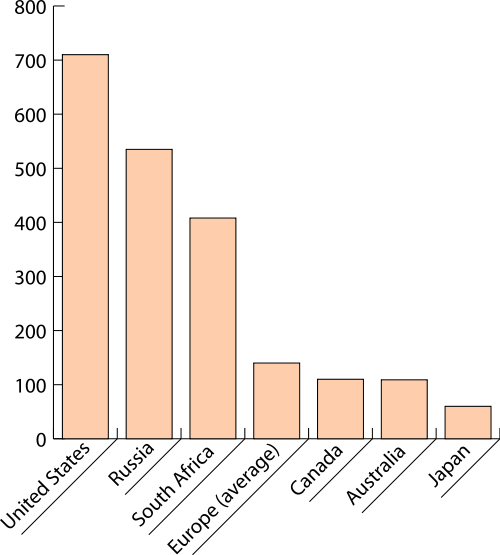
\includegraphics[width=\chartwidth,height=\chartheight]{incarceration}  
\source{Wikipedia}
\end{chart}

\begin{chart}{S}{ll}
\caption{Incarceration ratest across countries}
\label{chart:incarceration}
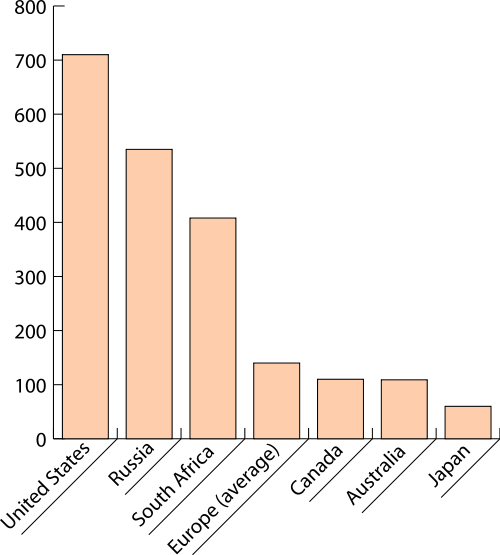
\includegraphics[width=\chartwidth,height=\chartheight]{incarceration}  
\source{Wikipedia}
\end{chart}

\begin{chart}{S}{lr}
\caption{Incarceration ratest across countries}
\label{chart:incarceration}
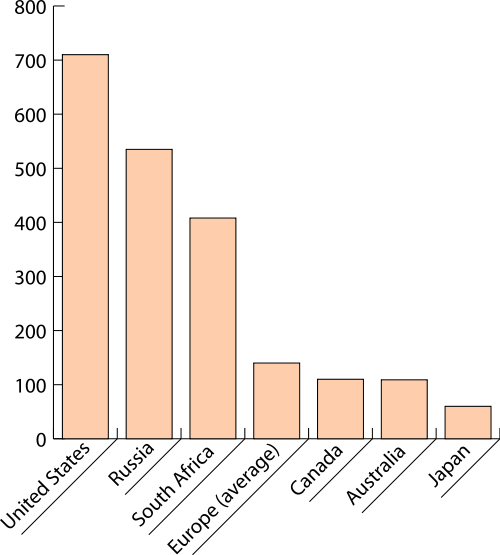
\includegraphics[width=\chartwidth,height=\chartheight]{incarceration}  
\source{Wikipedia}
\end{chart}

\begin{map}{W}{UL}
\caption{Ancient Roma  (Trajan times)}
\label{map:roma}
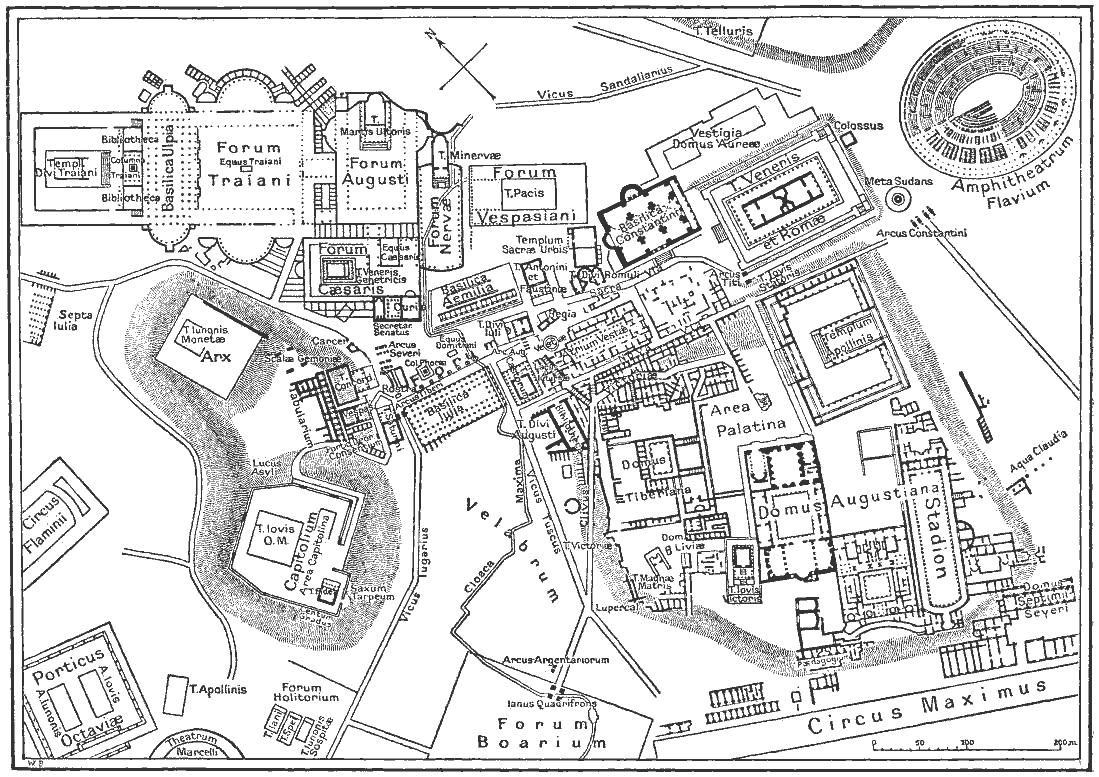
\includegraphics[width=\chartwidth,height=\chartheight]{Rome}
\source{Wikipedia}
\end{map}


\begin{map}{S}{LL}
\caption{Ancient Roma  (Trajan times)}
\label{map:roma}
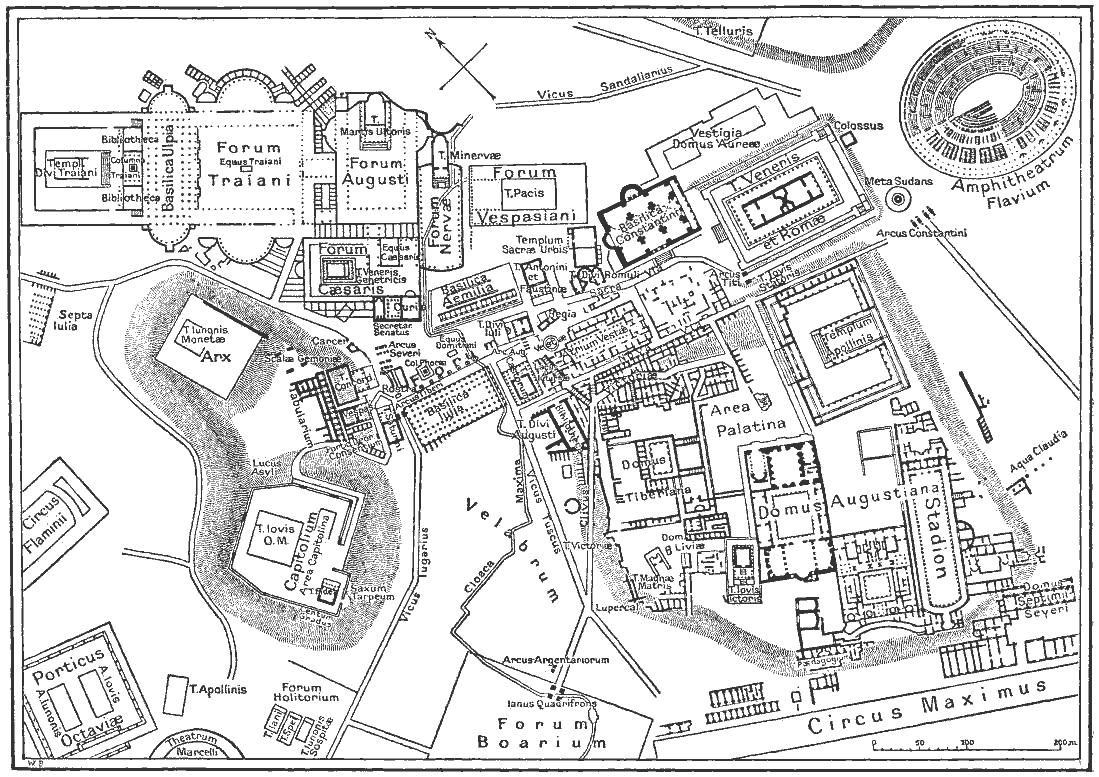
\includegraphics[width=\chartwidth,height=\chartheight]{Rome}
\source{Wikipedia}
\end{map}

\begin{map}{S}{LR}
\caption{Ancient Roma  (Trajan times)}
\label{map:roma}
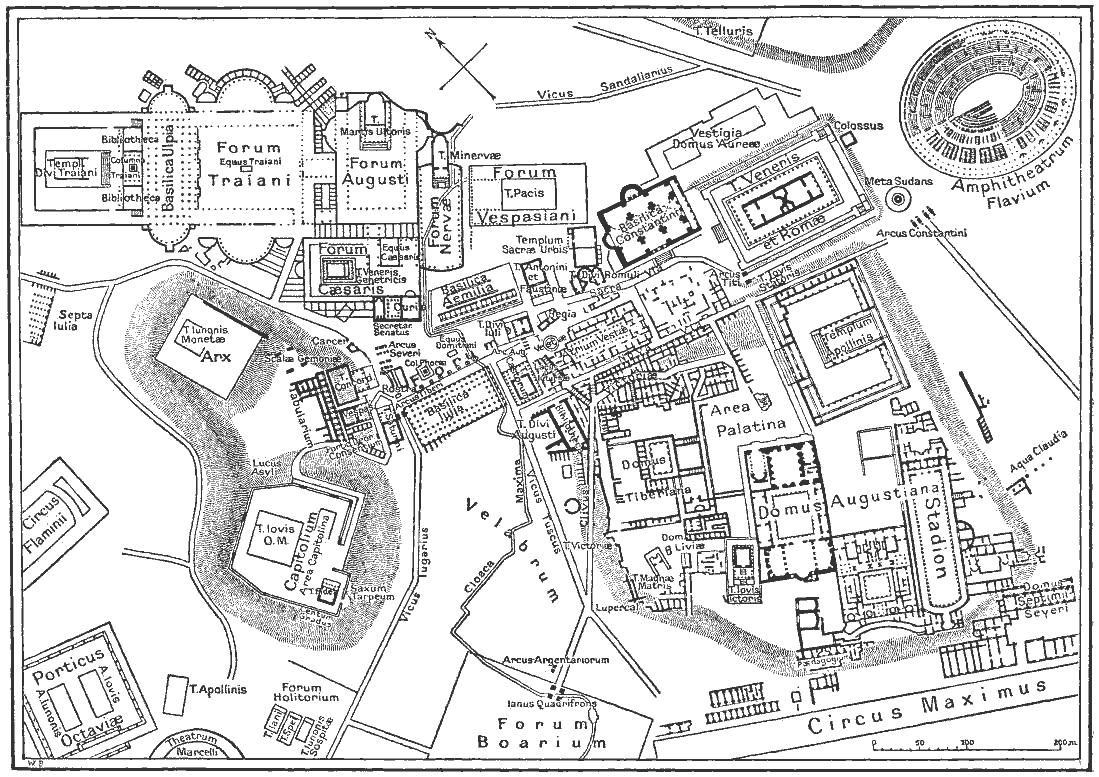
\includegraphics[width=\chartwidth,height=\chartheight]{Rome}
\source{Wikipedia}
\end{map}

\lipsum






\begin{tablepages}
\section{Inputs}
\small
% latex table generated in R 3.0.0 by xtable 1.7-1 package
% Tue Nov 19 17:29:13 2013
\begin{longtable}{p{3cm}<{\raggedright}d{7.0}d{2.1}d{1.1}d{2.1}d{2.1}d{2.1}d{2.1}d{1.1}d{2.1}}
\caption{Agricultural capital stock\label{T_P1.CAP.1}} \\ 
  
%first line header names
\rowcolor{@tableheadcolor}\cellcolor{white}
&
\multicolumn{9}{H}{\color{white}Gross capital stock} \\[-0.1ex]

%first line header horizontal lines
\hhline{%
	>{\arrayrulecolor{white}}~%
	>{\arrayrulecolor{@tableheadcolor}}|>{\arrayrulecolor{white}}---------%
	>{\arrayrulecolor{@tableheadcolor}}|%
}
%second line header names
\rowcolor{@tableheadcolor} \cellcolor{white} &
\multicolumn{3}{H}{\color{white}total} &
\multicolumn{6}{H}{\color{white}share} \\[-0.1ex]

%second line header horizontal lines
\hhline{%
	>{\arrayrulecolor{white}}~%
	>{\arrayrulecolor{@tableheadcolor}}|>{\arrayrulecolor{white}}---%
	>{\arrayrulecolor{@tableheadcolor}}|>{\arrayrulecolor{white}}------%
	>{\arrayrulecolor{@tableheadcolor}}|%
}
%third line header names
\rowcolor{@tableheadcolor} \cellcolor{white} &
\multicolumn{1}{C{1}}{\color{white} } &
\multicolumn{2}{H}{\color{white}p.a. growth} &
\multicolumn{1}{C{1}}{\color{white}land development} &
\multicolumn{1}{C{1}}{\color{white}plantation crops} &
\multicolumn{1}{C{1}}{\color{white}livestock fixed assets} &
\multicolumn{1}{C{1}}{\color{white}livestock inventory} &
\multicolumn{1}{C{1}}{\color{white}structures for livestock} &
\multicolumn{1}{C{1}}{\color{white}machinery \& equipment}  \\[-0.1ex]

%units in header 
\rowcolor{@tableheadcolor} \cellcolor{white} &
 \multicolumn{1}{C{1}}{\color{white}million US\$} &
 \multicolumn{1}{H}{\color{white}percent} &
 \multicolumn{1}{H}{\color{white}percent} &
 \multicolumn{1}{H}{\color{white}percent} &
 \multicolumn{1}{H}{\color{white}percent} &
 \multicolumn{1}{H}{\color{white}percent} &
 \multicolumn{1}{H}{\color{white}percent} &
 \multicolumn{1}{H}{\color{white}percent} &
 \multicolumn{1}{H}{\color{white}percent}\\ [-0.1ex]
%years in header
\rowcolor{@tableheadcolor} \cellcolor{white} &
 \multicolumn{1}{H}{\color{white}2007} &
 \multicolumn{1}{P{1.5cm}}{\color{white}1990-2000} &
 \multicolumn{1}{H}{\color{white}2000-07} &
 \multicolumn{1}{H}{\color{white}2007} &
 \multicolumn{1}{H}{\color{white}2007} &
 \multicolumn{1}{H}{\color{white}2007} &
 \multicolumn{1}{H}{\color{white}2007} &
 \multicolumn{1}{H}{\color{white}2007} &
 \multicolumn{1}{H}{\color{white}2007}\\ [-0.1ex]
\midrule
\endfirsthead
  \caption[]{Agricultural capital stock (continued)}\\
%first line header names
\rowcolor{@tableheadcolor}\cellcolor{white}
&
\multicolumn{9}{H}{\color{white}Gross capital stock} \\[-0.1ex]

%first line header horizontal lines
\hhline{%
	>{\arrayrulecolor{white}}~%
	>{\arrayrulecolor{@tableheadcolor}}|>{\arrayrulecolor{white}}---------%
	>{\arrayrulecolor{@tableheadcolor}}|%
}
%second line header names
\rowcolor{@tableheadcolor} \cellcolor{white} &
\multicolumn{3}{H}{\color{white}total} &
\multicolumn{6}{H}{\color{white}share} \\[-0.1ex]

%second line header horizontal lines
\hhline{%
	>{\arrayrulecolor{white}}~%
	>{\arrayrulecolor{@tableheadcolor}}|>{\arrayrulecolor{white}}---%
	>{\arrayrulecolor{@tableheadcolor}}|>{\arrayrulecolor{white}}------%
	>{\arrayrulecolor{@tableheadcolor}}|%
}
%third line header names
\rowcolor{@tableheadcolor} \cellcolor{white} &
\multicolumn{1}{C{1}}{\color{white} } &
\multicolumn{2}{H}{\color{white}p.a. growth} &
\multicolumn{1}{C{1}}{\color{white}land development} &
\multicolumn{1}{C{1}}{\color{white}plantation crops} &
\multicolumn{1}{C{1}}{\color{white}livestock fixed assets} &
\multicolumn{1}{C{1}}{\color{white}livestock inventory} &
\multicolumn{1}{C{1}}{\color{white}structures for livestock} &
\multicolumn{1}{C{1}}{\color{white}machinery \& equipment}  \\[-0.1ex]

%units in header 
\rowcolor{@tableheadcolor} \cellcolor{white} &
 \multicolumn{1}{C{1}}{\color{white}million US\$} &
 \multicolumn{1}{H}{\color{white}percent} &
 \multicolumn{1}{H}{\color{white}percent} &
 \multicolumn{1}{H}{\color{white}percent} &
 \multicolumn{1}{H}{\color{white}percent} &
 \multicolumn{1}{H}{\color{white}percent} &
 \multicolumn{1}{H}{\color{white}percent} &
 \multicolumn{1}{H}{\color{white}percent} &
 \multicolumn{1}{H}{\color{white}percent}\\ [-0.1ex]
%years in header
\rowcolor{@tableheadcolor} \cellcolor{white} &
 \multicolumn{1}{H}{\color{white}2007} &
 \multicolumn{1}{P{1.5cm}}{\color{white}1990-2000} &
 \multicolumn{1}{H}{\color{white}2000-07} &
 \multicolumn{1}{H}{\color{white}2007} &
 \multicolumn{1}{H}{\color{white}2007} &
 \multicolumn{1}{H}{\color{white}2007} &
 \multicolumn{1}{H}{\color{white}2007} &
 \multicolumn{1}{H}{\color{white}2007} &
 \multicolumn{1}{H}{\color{white}2007}\\ [-0.1ex]
\midrule 
\endhead
  \bottomrule
\endfoot
\tablemph{Regional office for the Near East} & 335\,938 & 1.9 & 1.2 & 61.9 & 3.3 & 21.9 & 3.9 & 2.3 & 6.7 \\ 
  \tablemph{Gulf Cooperation Council States and Yemen} & 41\,163 & 2.5 & 1.4 & 78.2 & 3.3 & 13.7 & 2.4 & 1.0 & 1.4 \\ 
     \hspace{2pt}\hangindent=4pt\relax Bahrain & 58 & 3.7 & -0.1 & 62.3 & 7.1 & 24.0 & 4.2 & 1.8 & 0.6 \\ 
     \hspace{2pt}\hangindent=4pt\relax Kuwait & 310 & 6.2 & 3.9 & 26.4 & 1.6 & 58.1 & 10.2 & 1.4 & 2.2 \\ 
     \hspace{2pt}\hangindent=4pt\relax Oman & 1\,329 & 2.9 & 0.5 & 42.3 & 4.2 & 41.2 & 7.3 & 3.7 & 1.3 \\ 
     \hspace{2pt}\hangindent=4pt\relax Qatar & 192 & 6.9 & -1.5 & 63.6 & 2.2 & 26.6 & 4.7 & 2.1 & 0.8 \\ 
     \hspace{2pt}\hangindent=4pt\relax Saudi Arabia & 23\,710 & 0.8 & 0.1 & 87.5 & 1.7 & 7.9 & 1.4 & 0.3 & 1.2 \\ 
     \hspace{2pt}\hangindent=4pt\relax United Arab Emirates & 3\,747 & 12.4 & 1.5 & 75.6 & 10.0 & 11.0 & 1.9 & 1.1 & 0.4 \\ 
     \hspace{2pt}\hangindent=4pt\relax Yemen & 11\,815 & 2.8 & 4.0 & 66.0 & 4.4 & 21.7 & 3.8 & 1.9 & 2.2 \\ 
  \tablemph{North Africa} & 62\,717 & 1.0 & 0.6 & 51.0 & 8.5 & 26.1 & 4.6 & 1.5 & 8.3 \\ 
     \hspace{2pt}\hangindent=4pt\relax Algeria & 14\,545 & 1.0 & 1.2 & 42.0 & 6.9 & 28.8 & 5.1 & 1.4 & 15.8 \\ 
     \hspace{2pt}\hangindent=4pt\relax Libya & 7\,531 & -0.1 & 0.7 & 64.6 & 5.6 & 15.4 & 2.7 & 0.5 & 11.1 \\ 
     \hspace{2pt}\hangindent=4pt\relax Mauritania & 4\,331 & 3.1 & 1.2 & 8.9 & 0.3 & 70.9 & 12.5 & 6.6 & 0.7 \\ 
     \hspace{2pt}\hangindent=4pt\relax Morocco & 26\,006 & 0.7 & 0.0 & 63.2 & 4.9 & 22.9 & 4.0 & 1.2 & 3.7 \\ 
     \hspace{2pt}\hangindent=4pt\relax Tunisia & 10\,304 & 1.8 & 0.8 & 40.5 & 25.5 & 19.2 & 3.4 & 0.9 & 10.5 \\ 
  \tablemph{Other Middle East countries} & 232\,058 & 2.1 & 1.4 & 61.9 & 1.9 & 22.2 & 3.9 & 2.8 & 7.2 \\ 
     \hspace{2pt}\hangindent=4pt\relax Egypt & 36\,793 & 2.3 & 1.5 & 73.6 & 2.3 & 15.1 & 2.7 & 2.3 & 4.0 \\ 
     \hspace{2pt}\hangindent=4pt\relax Iran (Islamic Republic of) & 85\,173 & 1.0 & 1.6 & 63.5 & 1.7 & 17.9 & 3.2 & 1.2 & 12.6 \\ 
     \hspace{2pt}\hangindent=4pt\relax Iraq & 31\,881 & -0.0 & 0.2 & 83.2 & 0.9 & 8.8 & 1.5 & 0.5 & 5.1 \\ 
     \hspace{2pt}\hangindent=4pt\relax Jordan & 1\,530 & 1.8 & 1.1 & 51.1 & 7.4 & 27.1 & 4.8 & 0.9 & 8.8 \\ 
     \hspace{2pt}\hangindent=4pt\relax Lebanon & 2\,845 & 0.6 & 0.1 & 73.2 & 16.8 & 6.5 & 1.1 & 0.4 & 2.0 \\ 
     \hspace{2pt}\hangindent=4pt\relax Sudan &  &  &  &  &  &  &  &  &  \\ 
     \hspace{2pt}\hangindent=4pt\relax Sudan (former) & 48\,106 & 4.5 & 1.4 & 29.4 & 0.4 & 50.9 & 9.0 & 9.0 & 1.3 \\ 
     \hspace{2pt}\hangindent=4pt\relax Syrian Arab Republic & 25\,731 & 4.1 & 2.4 & 73.9 & 4.2 & 11.2 & 2.0 & 0.5 & 8.3 \\ 
  \tablemph{Regional Office for Africa} & 430\,811 & 1.8 & 2.0 & 25.5 & 7.3 & 48.0 & 8.5 & 7.7 & 3.0 \\ 
  \tablemph{Regional Office for Asia and the Pacific} & 1\,719\,508 & 0.9 & 0.7 & 32.5 & 10.2 & 25.9 & 4.6 & 4.1 & 22.6 \\ 
  \tablemph{Regional Office for Europe and Central Asia} & 1\,239\,351 &  & -0.4 & 35.2 & 5.8 & 16.5 & 2.9 & 4.3 & 35.3 \\ 
  \tablemph{Regional Office for Latin America and the Caribbean} & 725\,911 & 0.5 & 0.9 & 24.3 & 6.9 & 47.1 & 8.3 & 5.2 & 8.1 \\ 
  \tablemph{World} & 4\,797\,327 & 0.6 & 0.6 & 31.0 & 7.6 & 26.8 & 4.7 & 5.4 & 24.5 \\ 
  \hline
\end{longtable}
  
\clearpage
% latex table generated in R 3.0.0 by xtable 1.7-1 package
% Tue Nov 19 17:35:30 2013
\begin{longtable}{p{3cm}<{\raggedright}d{2.0}d{3.0}d{3.0}d{2.0}d{2.0}d{2.0}d{2.0}d{2.1}d{2.1}}
\caption{Health and education\label{T_P2.HE.1}} \\ 
%first line header names
\rowcolor{@tableheadcolor}\cellcolor{white}
&
\multicolumn{1}{C{1}}{\color{white}Literacy rate} &
\multicolumn{2}{H}{\color{white}Primary completion rate} &
\multicolumn{4}{H}{\color{white}School enrollment} &
\multicolumn{2}{H}{\color{white}Health expenditure} \\[-0.1ex]

%first line header horizontal lines
\hhline{%
	>{\arrayrulecolor{white}}~%
	>{\arrayrulecolor{@tableheadcolor}}|>{\arrayrulecolor{white}}-%
	>{\arrayrulecolor{@tableheadcolor}}|>{\arrayrulecolor{white}}--%
	>{\arrayrulecolor{@tableheadcolor}}|>{\arrayrulecolor{white}}----%
	>{\arrayrulecolor{@tableheadcolor}}|>{\arrayrulecolor{white}}--%
	>{\arrayrulecolor{@tableheadcolor}}|%
}
%second line header names
\rowcolor{@tableheadcolor} \cellcolor{white} &
\multicolumn{1}{C{1}}{\color{white}adult female, \% of females ages 15 +} &
\multicolumn{2}{H}{\color{white}total} &
\multicolumn{4}{H}{\color{white}primary} &
\multicolumn{2}{H}{\color{white}share of GDP} \\[-0.1ex]

%second line header horizontal lines
\hhline{%
	>{\arrayrulecolor{white}}~%
	>{\arrayrulecolor{@tableheadcolor}}|>{\arrayrulecolor{white}}-%
	>{\arrayrulecolor{@tableheadcolor}}|>{\arrayrulecolor{white}}--%
	>{\arrayrulecolor{@tableheadcolor}}|>{\arrayrulecolor{white}}----%
	>{\arrayrulecolor{@tableheadcolor}}|>{\arrayrulecolor{white}}--%
	>{\arrayrulecolor{@tableheadcolor}}|%
}
%third line header names
\rowcolor{@tableheadcolor} \cellcolor{white} &
\multicolumn{1}{C{1}}{\color{white} } &
\multicolumn{2}{H}{\color{white} } &
\multicolumn{2}{H}{\color{white}female} &
\multicolumn{2}{H}{\color{white}male} &
\multicolumn{2}{H}{\color{white} } \\[-0.1ex]

%units in header 
\rowcolor{@tableheadcolor} \cellcolor{white} &
 \multicolumn{1}{H}{\color{white}percent} &
 \multicolumn{1}{H}{\color{white}percent} &
 \multicolumn{1}{H}{\color{white}percent} &
 \multicolumn{1}{H}{\color{white}percent} &
 \multicolumn{1}{H}{\color{white}percent} &
 \multicolumn{1}{H}{\color{white}percent} &
 \multicolumn{1}{H}{\color{white}percent} &
 \multicolumn{1}{H}{\color{white}percent} &
 \multicolumn{1}{H}{\color{white}percent}\\ [-0.1ex]
%years in header
\rowcolor{@tableheadcolor} \cellcolor{white} &
 \multicolumn{1}{H}{\color{white}2005-10*} &
 \multicolumn{1}{H}{\color{white}1990} &
 \multicolumn{1}{H}{\color{white}2010} &
 \multicolumn{1}{H}{\color{white}1990} &
 \multicolumn{1}{H}{\color{white}2010} &
 \multicolumn{1}{H}{\color{white}1990} &
 \multicolumn{1}{H}{\color{white}2010} &
 \multicolumn{1}{H}{\color{white}1995} &
 \multicolumn{1}{H}{\color{white}2010}\\ [-0.1ex]
\midrule
\endfirsthead
  \caption[]{Health and education (continued)}\\
%first line header names
\rowcolor{@tableheadcolor}\cellcolor{white}
&
\multicolumn{1}{C{1}}{\color{white}Literacy rate} &
\multicolumn{2}{H}{\color{white}Primary completion rate} &
\multicolumn{4}{H}{\color{white}School enrollment} &
\multicolumn{2}{H}{\color{white}Health expenditure} \\[-0.1ex]

%first line header horizontal lines
\hhline{%
	>{\arrayrulecolor{white}}~%
	>{\arrayrulecolor{@tableheadcolor}}|>{\arrayrulecolor{white}}-%
	>{\arrayrulecolor{@tableheadcolor}}|>{\arrayrulecolor{white}}--%
	>{\arrayrulecolor{@tableheadcolor}}|>{\arrayrulecolor{white}}----%
	>{\arrayrulecolor{@tableheadcolor}}|>{\arrayrulecolor{white}}--%
	>{\arrayrulecolor{@tableheadcolor}}|%
}
%second line header names
\rowcolor{@tableheadcolor} \cellcolor{white} &
\multicolumn{1}{C{1}}{\color{white}adult female, \% of females ages 15 +} &
\multicolumn{2}{H}{\color{white}total} &
\multicolumn{4}{H}{\color{white}primary} &
\multicolumn{2}{H}{\color{white}share of GDP} \\[-0.1ex]

%second line header horizontal lines
\hhline{%
	>{\arrayrulecolor{white}}~%
	>{\arrayrulecolor{@tableheadcolor}}|>{\arrayrulecolor{white}}-%
	>{\arrayrulecolor{@tableheadcolor}}|>{\arrayrulecolor{white}}--%
	>{\arrayrulecolor{@tableheadcolor}}|>{\arrayrulecolor{white}}----%
	>{\arrayrulecolor{@tableheadcolor}}|>{\arrayrulecolor{white}}--%
	>{\arrayrulecolor{@tableheadcolor}}|%
}
%third line header names
\rowcolor{@tableheadcolor} \cellcolor{white} &
\multicolumn{1}{C{1}}{\color{white} } &
\multicolumn{2}{H}{\color{white} } &
\multicolumn{2}{H}{\color{white}female} &
\multicolumn{2}{H}{\color{white}male} &
\multicolumn{2}{H}{\color{white} } \\[-0.1ex]

%units in header 
\rowcolor{@tableheadcolor} \cellcolor{white} &
 \multicolumn{1}{H}{\color{white}percent} &
 \multicolumn{1}{H}{\color{white}percent} &
 \multicolumn{1}{H}{\color{white}percent} &
 \multicolumn{1}{H}{\color{white}percent} &
 \multicolumn{1}{H}{\color{white}percent} &
 \multicolumn{1}{H}{\color{white}percent} &
 \multicolumn{1}{H}{\color{white}percent} &
 \multicolumn{1}{H}{\color{white}percent} &
 \multicolumn{1}{H}{\color{white}percent}\\ [-0.1ex]
%years in header
\rowcolor{@tableheadcolor} \cellcolor{white} &
 \multicolumn{1}{H}{\color{white}2005-10*} &
 \multicolumn{1}{H}{\color{white}1990} &
 \multicolumn{1}{H}{\color{white}2010} &
 \multicolumn{1}{H}{\color{white}1990} &
 \multicolumn{1}{H}{\color{white}2010} &
 \multicolumn{1}{H}{\color{white}1990} &
 \multicolumn{1}{H}{\color{white}2010} &
 \multicolumn{1}{H}{\color{white}1995} &
 \multicolumn{1}{H}{\color{white}2010}\\ [-0.1ex]
\midrule 
\endhead
  \bottomrule
\endfoot
\tablemph{Africa} &  &  &  &  &  &  &  & 5.1 & 6.0 \\ 
  \tablemph{North Africa} &  &  & 96 &  &  &  &  & 4.1 & 5.2 \\ 
     \hspace{2pt}\hangindent=4pt\relax Algeria & 64 & 81 & 96 & 81 & 95 & 94 & 97 & 4.2 & 4.3 \\ 
     \hspace{2pt}\hangindent=4pt\relax Egypt & 64 &  & 101 &  &  &  &  & 3.9 & 4.7 \\ 
     \hspace{2pt}\hangindent=4pt\relax Libya & 83 &  &  &  &  &  &  & 3.5 &  \\ 
     \hspace{2pt}\hangindent=4pt\relax Morocco & 44 & 52 & 85 & 46 & 93 & 67 & 95 & 3.9 & 5.9 \\ 
     \hspace{2pt}\hangindent=4pt\relax Sudan &  &  &  &  &  &  &  &  & 7.2 \\ 
     \hspace{2pt}\hangindent=4pt\relax Tunisia & 71 & 80 &  & 87 &  & 97 &  & 5.8 & 5.7 \\ 
  \tablemph{Regional Office for Africa} &  &  & 67 &  &  &  &  & 5.7 & 6.5 \\ 
  \tablemph{Central Africa} &  &  & 60 &  &  &  &  & 3.7 & 4.6 \\ 
     \hspace{2pt}\hangindent=4pt\relax Cameroon & 63 & 54 & 79 & 67 & 85 & 76 & 98 & 3.9 & 5.1 \\ 
     \hspace{2pt}\hangindent=4pt\relax Central African Republic & 43 & 30 & 41 & 46 & 60 & 69 & 81 & 3.9 & 3.8 \\ 
     \hspace{2pt}\hangindent=4pt\relax Chad & 24 & 17 & 35 &  &  &  &  & 5.8 & 4.0 \\ 
     \hspace{2pt}\hangindent=4pt\relax Congo &  & 60 & 71 &  & 89 &  & 92 & 3.2 & 2.3 \\ 
     \hspace{2pt}\hangindent=4pt\relax Democratic Republic of the Congo & 57 &  & 59 &  &  &  &  & 3.6 & 7.5 \\ 
     \hspace{2pt}\hangindent=4pt\relax Equatorial Guinea & 91 &  & 52 &  & 56 &  & 57 & 5.9 & 4.2 \\ 
     \hspace{2pt}\hangindent=4pt\relax Gabon & 85 &  &  &  &  &  &  & 3.0 & 3.5 \\ 
     \hspace{2pt}\hangindent=4pt\relax Sao Tome and Principe & 85 & 79 & 85 &  &  &  &  &  & 7.5 \\ 
  \tablemph{East Africa} &  &  & 68 &  &  &  &  & 3.9 & 5.7 \\ 
     \hspace{2pt}\hangindent=4pt\relax Burundi & 62 & 41 & 56 &  &  &  &  & 5.5 & 9.1 \\ 
     \hspace{2pt}\hangindent=4pt\relax Djibouti &  & 32 &  & 25 &  & 33 &  & 4.0 &  \\ 
     \hspace{2pt}\hangindent=4pt\relax Eritrea & 58 &  & 40 &  & 31 &  & 36 & 4.5 & 2.9 \\ 
     \hspace{2pt}\hangindent=4pt\relax Ethiopia & 29 &  & 62 &  & 79 &  & 84 & 2.8 & 4.8 \\ 
     \hspace{2pt}\hangindent=4pt\relax Kenya & 84 &  &  &  &  &  &  & 4.3 & 4.4 \\ 
     \hspace{2pt}\hangindent=4pt\relax Rwanda & 68 & 45 & 70 &  &  &  &  & 4.5 & 10.4 \\ 
     \hspace{2pt}\hangindent=4pt\relax Somalia &  &  &  &  &  &  &  &  &  \\ 
     \hspace{2pt}\hangindent=4pt\relax South Sudan &  &  &  &  &  &  &  &  & 2.1 \\ 
     \hspace{2pt}\hangindent=4pt\relax Sudan (former) & 62 &  &  &  &  &  &  & 3.4 &  \\ 
     \hspace{2pt}\hangindent=4pt\relax Uganda & 65 &  & 57 &  & 92 &  & 90 & 5.8 & 9.2 \\ 
     \hspace{2pt}\hangindent=4pt\relax United Republic of Tanzania & 67 &  & 90 & 52 &  & 51 &  & 3.6 & 7.2 \\ 
  \tablemph{Southern Africa} &  &  & 68 &  &  &  &  & 6.7 & 7.4 \\ 
     \hspace{2pt}\hangindent=4pt\relax Angola & 58 &  & 47 &  & 78 &  & 93 & 5.1 & 3.4 \\ 
     \hspace{2pt}\hangindent=4pt\relax Botswana & 85 & 89 &  & 89 &  & 82 &  & 4.2 & 5.1 \\ 
     \hspace{2pt}\hangindent=4pt\relax Comoros & 70 &  &  &  &  &  &  & 4.7 & 5.3 \\ 
     \hspace{2pt}\hangindent=4pt\relax Lesotho & 96 & 58 & 70 & 78 & 75 & 63 & 72 & 8.1 & 11.5 \\ 
     \hspace{2pt}\hangindent=4pt\relax Madagascar & 62 & 36 & 72 & 69 &  & 70 &  & 2.8 & 3.6 \\ 
     \hspace{2pt}\hangindent=4pt\relax Malawi & 68 & 28 & 68 &  &  &  &  & 5.0 & 8.4 \\ 
     \hspace{2pt}\hangindent=4pt\relax Mauritius & 86 & 111 &  &  &  &  &  & 3.6 & 6.2 \\ 
     \hspace{2pt}\hangindent=4pt\relax Mozambique & 43 & 27 & 61 &  & 89 &  & 94 & 5.3 & 6.3 \\ 
     \hspace{2pt}\hangindent=4pt\relax Namibia & 88 &  & 81 & 83 & 87 & 76 & 83 & 6.2 & 5.5 \\ 
     \hspace{2pt}\hangindent=4pt\relax Seychelles & 92 &  & 133 &  &  &  &  & 5.2 & 3.3 \\ 
     \hspace{2pt}\hangindent=4pt\relax South Africa & 87 &  &  &  &  &  &  & 7.4 & 8.7 \\ 
     \hspace{2pt}\hangindent=4pt\relax Swaziland & 87 & 63 & 77 & 76 &  & 72 &  & 5.0 & 7.8 \\ 
     \hspace{2pt}\hangindent=4pt\relax Zambia & 62 &  & 103 &  & 92 &  & 90 & 5.6 & 6.0 \\ 
     \hspace{2pt}\hangindent=4pt\relax Zimbabwe & 90 &  &  &  &  &  &  & 0.1 &  \\ 
  \tablemph{West Africa} &  &  & 68 &  &  &  &  & 4.8 & 5.7 \\ 
     \hspace{2pt}\hangindent=4pt\relax Benin & 30 & 19 & 70 & 28 &  & 55 &  & 4.7 & 4.3 \\ 
     \hspace{2pt}\hangindent=4pt\relax Burkina Faso & 22 & 18 & 45 &  & 56 &  & 60 & 4.3 & 7.4 \\ 
     \hspace{2pt}\hangindent=4pt\relax Cabo Verde & 79 & 57 & 99 &  & 92 &  & 94 & 5.3 & 4.8 \\ 
     \hspace{2pt}\hangindent=4pt\relax C\^{o}te d'Ivoire & 47 & 40 &  &  &  &  &  & 5.1 & 6.2 \\ 
     \hspace{2pt}\hangindent=4pt\relax Gambia & 40 &  & 70 &  & 67 &  & 64 & 3.3 & 4.4 \\ 
     \hspace{2pt}\hangindent=4pt\relax Ghana & 61 &  &  &  &  &  &  & 5.3 & 5.2 \\ 
     \hspace{2pt}\hangindent=4pt\relax Guinea & 30 & 21 & 64 & 18 & 70 & 36 & 83 & 5.5 & 6.2 \\ 
     \hspace{2pt}\hangindent=4pt\relax Guinea-Bissau & 41 &  & 68 &  & 72 &  & 75 & 6.4 & 7.0 \\ 
     \hspace{2pt}\hangindent=4pt\relax Liberia & 57 &  &  &  &  &  &  & 0.0 & 16.4 \\ 
     \hspace{2pt}\hangindent=4pt\relax Mali & 20 &  & 55 &  & 57 &  & 66 & 5.2 & 6.5 \\ 
     \hspace{2pt}\hangindent=4pt\relax Mauritania & 51 & 29 &  &  & 76 &  & 72 & 4.8 & 6.1 \\ 
     \hspace{2pt}\hangindent=4pt\relax Niger & 15 & 17 & 41 & 18 & 51 & 29 & 63 & 3.4 & 4.8 \\ 
     \hspace{2pt}\hangindent=4pt\relax Nigeria & 50 &  & 74 &  & 55 &  & 60 & 4.5 & 5.4 \\ 
     \hspace{2pt}\hangindent=4pt\relax Senegal & 39 & 43 & 59 & 39 & 78 & 53 & 73 & 3.9 & 5.8 \\ 
     \hspace{2pt}\hangindent=4pt\relax Sierra Leone & 31 &  &  &  &  &  &  & 15.3 & 20.8 \\ 
     \hspace{2pt}\hangindent=4pt\relax Togo & 44 & 38 & 74 & 55 &  & 79 &  & 4.6 & 7.5 \\ 
  \tablemph{CEMAC} &  & 42 & 61 &  &  &  &  & 3.7 & 4.0 \\ 
  \tablemph{CEN-SAD} &  &  &  &  &  &  &  & 4.2 & 5.5 \\ 
  \tablemph{COMESA} &  &  &  &  &  &  &  & 3.7 & 5.4 \\ 
  \tablemph{ECCAS} &  &  & 57 &  &  &  &  & 4.0 & 4.0 \\ 
  \tablemph{ECOWAS} &  &  & 68 &  &  &  &  & 4.8 & 5.7 \\ 
  \tablemph{IGAD} &  &  &  &  &  &  &  & 3.9 & 5.9 \\ 
  \tablemph{SADC} &  &  & 70 &  &  &  &  & 6.5 & 7.4 \\ 
  \tablemph{UEMOA} &  & 30 & 54 &  &  &  &  & 4.6 & 6.1 \\ 
  \tablemph{UMA} &  & 67 &  &  &  &  &  & 4.2 & 5.0 \\ 
  \tablemph{Regional Office for Asia and the Pacific} &  &  &  &  &  &  &  & 5.8 & 6.4 \\ 
  \tablemph{Regional Office for Europe and Central Asia} &  &  & 99 &  &  &  &  & 8.4 & 9.8 \\ 
  \tablemph{Regional Office for Latin America and the Caribbean} &  &  & 102 &  &  &  &  & 6.5 & 7.6 \\ 
  \tablemph{Regional Office for the Near East} &  &  &  &  &  &  &  & 3.8 & 4.6 \\ 
  \tablemph{World} &  &  &  &  &  &  &  & 8.8 & 10.3 \\ 
  \hline
\end{longtable}

\end{tablepages}


\metadatasection{Indicators}

\begin{metadata}{Agricultural population}

\key{agripop}
Agricultural population is defined as all persons depending for their livelihood on agriculture, hunting, fishing and forestry. It comprises all persons economically active in agriculture as well as their non-working dependents. It is not necessary that this referred population exclusively come from rural population.
\source{\href{http://www.fao.org/economic/ess/en/}{Statistics
    Division} (\href{http://faostat.fao.org}{FAOSTAT})} 
\owner{\href{http://www.fao.org}{FAO}} 
\end{metadata}


\begin{metadata}{Core}
  \lipsum[1]
\end{metadata}

\faoset{bgcolor=orange,icon=icons/hunger}
\part{Hunger Dimensions}
\lipsum
\EndPartIntro
\lipsum[1-2]

\faoset{bgcolor=red!70!blue,icon=icons/feeding}
\part[Feeding the world]{Feeding\\ the world}
\lipsum
\EndPartIntro

\lipsum[2-12]

\faoset{bgcolor=green!75!blue,icon=icons/sustainability}
\part[Sustainability dimensions]{Sustain\-ability dimensions}
\lipsum
\EndPartIntro

\begin{map}{S}{ll}
\caption{Ancient Roma  (Trajan times)}
\label{map:roma}
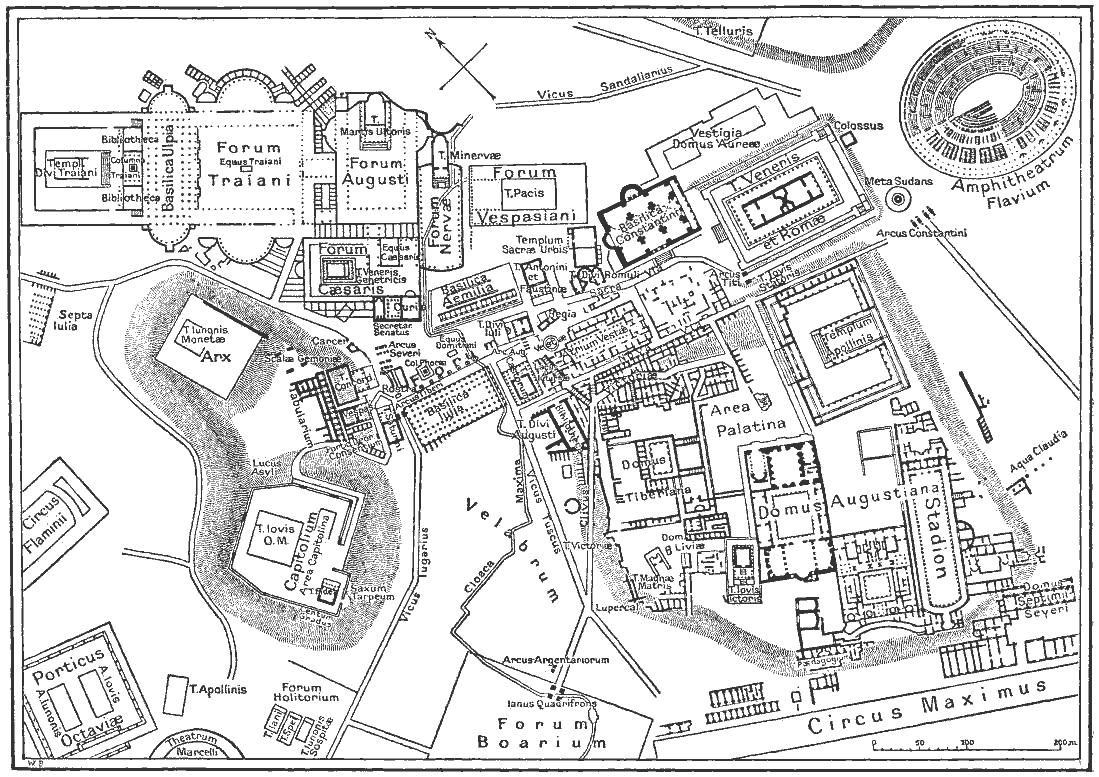
\includegraphics[width=\chartwidth,height=\chartheight]{Rome}
\source{Wikipedia}
\end{map}



\end{document}


